% !TeX program = pdflatex
\documentclass{beamer}
\usepackage[utf8]{inputenc}
\usepackage[polish]{babel}
\usepackage[T1]{fontenc}
\usepackage{tikz}
\usetikzlibrary{positioning, arrows.meta, decorations.pathreplacing, calc}
\usepackage{graphicx}
\usepackage{hyperref}
\usepackage{biblatex}
\usepackage{amsmath, amssymb}
\usepackage{caption}
\addbibresource{references.bib}

% Global font settings
\usepackage{lmodern}  % Latin Modern font
\usefonttheme{professionalfonts}  % Use professional fonts
\setbeamerfont{title}{size=\large,series=\bfseries}
\setbeamerfont{frametitle}{size=\normalsize,series=\bfseries}
\setbeamerfont{normal text}{size=\small}

% Ulepszony motyw i kolory
\usetheme{Madrid}
\usecolortheme{dolphin}
\setbeamertemplate{navigation symbols}{}
\setbeamertemplate{footline}[frame number]

% Lepsze style dla diagramów
\tikzset{
  block/.style={
    draw,
    rectangle,
    rounded corners,
    minimum width=2cm,
    minimum height=1cm,
    align=center,
    fill=blue!10
  },
  annotation/.style={
    draw=red,
    thick,
    -Stealth
  }
}

% Definicja środowiska formula
\newenvironment{formula}{%
  \begin{tcolorbox}[colback=yellow!10!white, colframe=black!60, boxrule=0.5pt, arc=3mm, boxsep=3pt]%
}{%
  \end{tcolorbox}%
}

% Dodanie pakietu tcolorbox
\usepackage{tcolorbox}

\title{Generowanie cyfr pisanych odręcznie na bazie sieci neuronowej o architekturze autoencodera}
\subtitle{Analiza i implementacja różnych modeli generatywnych}
\author{Prowadzący: Adam Świtoński}
\institute{Politechnika Śląska}
\date{Maj 2025}

\begin{document}

\begin{frame}
  \titlepage
\end{frame}

\begin{frame}{Plan prezentacji}
  \tableofcontents
\end{frame}

\begin{frame}{Opis projektu}
  \begin{block}{Cel projektu}
    Zastosowanie sieci neuronowej o architekturze autoencodera do generowania niskorozdzielczych obrazów cyfr pisanych odręcznie.
  \end{block}
  
  \begin{itemize}
    \item Trenowanie różnych wariantów autoencoder'a
    \item Generowanie nowych cyfr poprzez podawanie losowych wartości na wejście dekodera
    \item Badanie wpływu struktury sieci (liczba warstw, liczba neuronów) oraz parametrów uczenia
    \item Wykorzystanie zbioru danych MNIST
  \end{itemize}
  
  \begin{block}{Rozważane warianty}
    Klasyczny autoencoder, wariacyjny autoencoder (VAE), GAN, Diffusion, VQ-VAE, Conditional VAE
  \end{block}
\end{frame}

\begin{frame}
  \frametitle{Zbiór danych MNIST}
  
  \textbf{Charakterystyka zbioru MNIST:}
  \begin{itemize}
      \item Standardowy zbiór danych do rozpoznawania odręcznie pisanych cyfr
      \item 60 000 obrazów treningowych
      \item 10 000 obrazów testowych
      \item Obrazy czarno-białe o wymiarach 28 $\times$ 28 pikseli
      \item 10 klas (cyfry od 0 do 9)
      \item Każdy piksel reprezentowany jako wartość od 0 (biały) do 255 (czarny)
  \end{itemize}

  \vspace{0.5cm}
  \begin{center}
    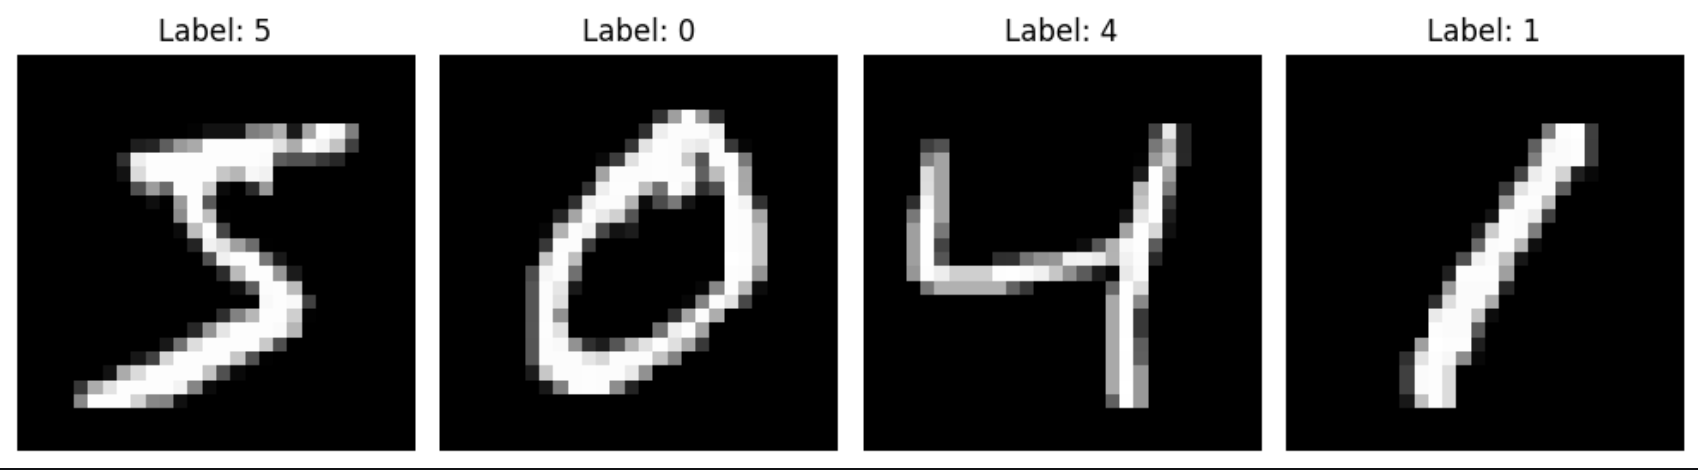
\includegraphics[width=0.5\textwidth]{img/mnist_example.png}\\
    \captionof{figure}{Przykładowe cyfry ze zbioru MNIST}
  \end{center}
\end{frame}

\begin{frame}
  \frametitle{Dlaczego MNIST?}
  
  \begin{columns}[T]
  \begin{column}{0.6\textwidth}
      \textbf{Zalety zbioru MNIST:}
      \begin{itemize}
          \item Idealny do demonstracji modeli generatywnych ze względu na prostotę
          \item Pozwala na szybkie eksperymenty (mała rozdzielczość obrazów)
          \item Łatwa interpretacja wyników (ludzie bez trudu rozpoznają cyfry)
          \item Umożliwia bezpośrednie porównanie z wynikami z literatury
      \end{itemize}
  \end{column}
  
  \begin{column}{0.4\textwidth}
      \vspace{0.5cm}
      \begin{tcolorbox}[colback=yellow!10!white, colframe=black!60, boxrule=0.5pt, arc=3mm]
          \centering
          \textbf{Balans między:}
          \begin{itemize}
              \item Złożonością modelu
              \item Czasem treningu
              \item Jakością wyników
          \end{itemize}
      \end{tcolorbox}
  \end{column}
  \end{columns}
\end{frame}

% --- MODELE ---

\section{Modele}

% AUTOENCODER
\begin{frame}{Autoencoder}
  \begin{columns}
    \begin{column}{0.6\textwidth}
    \textbf{Autoencoder} to rodzaj sieci neuronowej, która uczy się kompresować dane wejściowe do reprezentacji o niższym wymiarze (kod), a następnie rekonstruować oryginalne dane z tej reprezentacji.
    
    \medskip
    \textbf{Zastosowania:}
    \begin{itemize}
    \item Redukcja wymiarowości
    \item Denoising (odszumianie)
    \item Generowanie nowych danych
    \end{itemize}
    
    \textbf{Zalety:} prostota, szybki trening, interpretowalność
    
    \textbf{Wady:} ograniczona zdolność generatywna, brak kontroli nad rozkładem latentnym
    
    \textbf{Bibliografia:} \cite{hinton2006reducing}
    \end{column}
    \begin{column}{0.4\textwidth}
    \centering
    \begin{tikzpicture}[scale=0.6, transform shape]
    \node[block] (input) at (0,0) {Wejście};
    \node[block, below=0.8cm of input] (enc) {Enkoder};
    \node[block, below=0.8cm of enc] (code) {Kod};
    \node[block, below=0.8cm of code] (dec) {Dekoder};
    \node[block, below=0.8cm of dec] (output) {Wyjście};
    
    \draw[->, thick] (input) -- (enc);
    \draw[->, thick] (enc) -- (code);
    \draw[->, thick] (code) -- (dec);
    \draw[->, thick] (dec) -- (output);
    \end{tikzpicture}
    \end{column}
  \end{columns}
\end{frame}

\begin{frame}{Autoencoder - Funkcja straty (1/2)}
  \begin{columns}
    \begin{column}{0.5\textwidth}
      \centering
      \begin{tikzpicture}[scale=0.6, transform shape]
        \node[block] (input) at (0,0) {$x$};
        \node[block, below=0.8cm of input] (enc) {Enkoder $f(x)$};
        \node[block, below=0.8cm of enc] (code) {$z = f(x)$};
        \node[block, below=0.8cm of code] (dec) {Dekoder $g(z)$};
        \node[block, below=0.8cm of dec] (output) {$\hat{x} = g(f(x))$};
        
        \draw[->, thick] (input) -- (enc);
        \draw[->, thick] (enc) -- (code);
        \draw[->, thick] (code) -- (dec);
        \draw[->, thick] (dec) -- (output);
      \end{tikzpicture}
    \end{column}
    \begin{column}{0.5\textwidth}
      \textbf{Struktura Autoencodera:}
      \medskip
      Autoencoder składa się z enkodera, który kompresuje dane wejściowe do reprezentacji latentnej, oraz dekodera, który rekonstruuje dane z tej reprezentacji.
      
      \medskip
      Kluczowe elementy to dane wejściowe $x$, reprezentacja latentna $z$, oraz rekonstrukcja $\hat{x}$.
    \end{column}
  \end{columns}
\end{frame}

\begin{frame}{Autoencoder - Funkcja straty (2/2)}
  \begin{columns}
    \begin{column}{0.5\textwidth}
      \begin{tcolorbox}[colback=yellow!10!white, colframe=black!60, boxrule=0.5pt, arc=3mm]
        \begin{align*}
          \mathcal{L}_{AE} &= \|x - \hat{x}\|^2 \\
          &= \|x - g(f(x))\|^2
        \end{align*}
      \end{tcolorbox}
    \end{column}
    \begin{column}{0.5\textwidth}
      \textbf{Objaśnienie funkcji straty:}
      \medskip
      gdzie:
      \begin{itemize}
        \item $x$ - dane wejściowe (obraz)
        \item $f(x)$ - funkcja enkodera
        \item $z = f(x)$ - reprezentacja latentna
        \item $g(z)$ - funkcja dekodera
        \item $\hat{x} = g(f(x))$ - rekonstrukcja
      \end{itemize}
      
      Funkcja straty to typowo błąd średniokwadratowy (MSE) lub binary cross-entropy dla obrazów.
    \end{column}
  \end{columns}
\end{frame}

% VAE
\begin{frame}{Wariacyjny Autoencoder (VAE)}
  \begin{columns}
    \begin{column}{0.6\textwidth}
    \textbf{VAE} to probabilistyczne rozszerzenie autoencodera, które modeluje rozkład latentny danych.
    
    \medskip
    \textbf{Kluczowe cechy:}
    \begin{itemize}
    \item Modelowanie rozkładu latentnego ($\mu$, $\sigma$)
    \item Regularyzacja poprzez KL-dywergencję
    \item Generowanie nowych próbek przez próbkowanie
    \end{itemize}
    
    \textbf{Zalety:} generatywność, ciągła przestrzeń latentna, możliwość interpolacji
    
    \textbf{Wady:} rozmyte próbki, trudność w trenowaniu
    
    \textbf{Bibliografia:} \cite{kingma2013auto}
    \end{column}
    \begin{column}{0.4\textwidth}
    \centering
    \begin{tikzpicture}[scale=0.6, transform shape]
    \node[block] (input) at (0,0) {Wejście};
    \node[block, below=0.8cm of input] (enc) {Enkoder};
    \node[block, below=0.8cm of enc] (mu) {$\mu$, $\sigma$};
    \node[block, below=0.8cm of mu] (dec) {Dekoder};
    \node[block, below=0.8cm of dec] (output) {Wyjście};
    
    \draw[->, thick] (input) -- (enc);
    \draw[->, thick] (enc) -- (mu);
    \draw[->, thick] (mu) -- (dec);
    \draw[->, thick] (dec) -- (output);
    \end{tikzpicture}
    \end{column}
  \end{columns}
\end{frame}

\begin{frame}{Wariacyjny Autoencoder (VAE) - Funkcja straty (1/2)}
  \begin{columns}
    \begin{column}{0.5\textwidth}
      \centering
      \begin{tikzpicture}[scale=0.6, transform shape]
        \node[block] (input) at (0,0) {$x$};
        \node[block, right=0.6cm of input] (cond) {$y$ (etykieta)};
        \node[block, below=0.8cm of input] (concat1) {Konkatenacja};
        \draw[->, thick] (input) -- (concat1);
        \draw[->, thick] (cond) -- (concat1);
        
        \node[block, below=0.8cm of concat1] (enc) {Enkoder};
        \node[block, below=0.8cm of enc] (params) {$\mu(x), \sigma(x)$};
        \node[block, below=0.8cm of params] (sample) {$z \sim \mathcal{N}(\mu, \sigma^2)$};
        
        \node[block, below=0.8cm of sample] (concat2) {Konkatenacja};
        \draw[->, thick] (cond) to [out=270,in=0] (concat2);
        \draw[->, thick] (sample) -- (concat2);
        
        \node[block, below=0.8cm of concat2] (dec) {Dekoder};
        \node[block, below=0.8cm of dec] (output) {$\hat{x} = g(z,y)$};
        
        \draw[->, thick] (concat1) -- (enc);
        \draw[->, thick] (enc) -- (params);
        \draw[->, thick] (params) -- (sample);
        \draw[->, thick] (concat2) -- (dec);
        \draw[->, thick] (dec) -- (output);
      \end{tikzpicture}
    \end{column}
    \begin{column}{0.5\textwidth}
      \textbf{Struktura Conditional VAE:}
      \medskip
      Conditional VAE uwzględnia etykietę $y$ (np. klasę cyfry) podczas kodowania i dekodowania, co pozwala na kontrolowanie generowanych danych.
      
      \medskip
      Etykieta jest konkatenowana zarówno z danymi wejściowymi, jak i z próbkowaną reprezentacją latentną $z$.
    \end{column}
  \end{columns}
\end{frame}

\begin{frame}{Conditional VAE - Funkcja straty (2/2)}
  \begin{columns}
    \begin{column}{0.5\textwidth}
      \begin{tcolorbox}[colback=yellow!10!white, colframe=black!60, boxrule=0.5pt, arc=3mm]
        \begin{align*}
          \mathcal{L}_{CVAE} &= \underbrace{\|x - \hat{x}\|^2}_{\text{Rekonstrukcja}} + \\
          &\underbrace{\beta \cdot D_{KL}(q(z|x,y) \| p(z|y))}_{\text{Regularyzacja KL}}
        \end{align*}
      \end{tcolorbox}
    \end{column}
    \begin{column}{0.5\textwidth}
      \textbf{Objaśnienie funkcji straty:}
      \medskip
      gdzie:
      \begin{itemize}
        \item $q(z|x,y) = \mathcal{N}(z; \mu(x,y), \sigma^2(x,y))$
        \item $p(z|y)$ - warunkowy rozkład a priori
        \item $y$ - etykieta klasy (np. cyfra 0-9)
      \end{itemize}
      
      \medskip
      Podczas generowania:
      \begin{itemize}
        \item Wybierz etykietę $y$ (np. "3")
        \item Próbkuj $z \sim \mathcal{N}(0, I)$
        \item Wygeneruj $\hat{x} = g(z, y)$
      \end{itemize}
    \end{column}
  \end{columns}
\end{frame}

% VQ-VAE
\begin{frame}{VQ-VAE}
  \begin{columns}
    \begin{column}{0.6\textwidth}
    \textbf{VQ-VAE} to autoencoder, w którym przestrzeń latentna jest kwantyzowana do skończonego zbioru wektorów (słownik kodów).
    
    \medskip
    \textbf{Kluczowe cechy:}
    \begin{itemize}
    \item Dyskretna przestrzeń latentna
    \item Kwantyzacja wektorowa
    \item Słownik kodowy
    \end{itemize}
    
    \textbf{Zalety:} dyskretna reprezentacja, dobre wyniki w generowaniu sekwencji
    
    \textbf{Wady:} trudność w trenowaniu, konieczność doboru rozmiaru słownika
    
    \textbf{Bibliografia:} \cite{van2017neural}
    \end{column}
    \begin{column}{0.4\textwidth}
    \centering
    \begin{tikzpicture}[scale=0.6, transform shape]
    \node[block] (input) at (0,0) {Wejście};
    \node[block, below=0.8cm of input] (enc) {Enkoder};
    \node[block, below=0.8cm of enc] (quant) {Kwantyzacja};
    \node[block, below=0.8cm of quant] (dec) {Dekoder};
    \node[block, below=0.8cm of dec] (output) {Wyjście};
    
    \draw[->, thick] (input) -- (enc);
    \draw[->, thick] (enc) -- (quant);
    \draw[->, thick] (quant) -- (dec);
    \draw[->, thick] (dec) -- (output);
    \end{tikzpicture}
    \end{column}
  \end{columns}
\end{frame}

\begin{frame}{VQ-VAE - Funkcja straty (1/2)}
  \begin{columns}
    \begin{column}{0.5\textwidth}
      \begin{tikzpicture}[scale=0.6, transform shape]
        \node[block] (input) at (0,0) {$x$};
        \node[block, below=0.8cm of input] (enc) {Enkoder $f(x)$};
        \node[block, below=0.8cm of enc] (ze) {$z_e = f(x)$};
        
        \node[block, right=1.5cm of ze] (codebook) {Słownik kodów\\$\{e_k\}_{k=1}^K$};
        
        \node[block, below=0.8cm of ze] (zq) {$z_q = e_k$, gdzie $k = \arg\min_j \|z_e - e_j\|$};
        \node[block, below=0.8cm of zq] (dec) {Dekoder $g(z_q)$};
        \node[block, below=0.8cm of dec] (output) {$\hat{x} = g(z_q)$};
        
        \draw[->, thick] (input) -- (enc);
        \draw[->, thick] (enc) -- (ze);
        \draw[->, thick] (ze) -- (zq);
        \draw[->, thick] (codebook) -- node[midway, above] {wybierz} (zq);
        \draw[->, thick] (zq) -- (dec);
        \draw[->, thick] (dec) -- (output);
      \end{tikzpicture}
    \end{column}
    \begin{column}{0.5\textwidth}
      \textbf{Struktura VQ-VAE:}
      \medskip
      VQ-VAE kwantyzuje wyjście enkodera $z_e$ do najbliższego wektora $z_q$ ze słownika kodów, co prowadzi do dyskretnej reprezentacji latentnej.
      
      \medskip
      Słownik kodów jest kluczowym elementem, który pozwala na wybór odpowiedniego wektora podczas procesu kwantyzacji.
    \end{column}
  \end{columns}
\end{frame}

\begin{frame}{VQ-VAE - Funkcja straty (2/2)}
  \begin{columns}
    \begin{column}{0.5\textwidth}
      \begin{tcolorbox}[colback=yellow!10!white, colframe=black!60, boxrule=0.5pt, arc=3mm]
        \begin{align*}
          \mathcal{L}_{VQ-VAE} &= \underbrace{\|x - \hat{x}\|^2}_{\text{Rekonstrukcja}} + \\
          &\underbrace{\|sg[z_e] - e\|^2}_{\text{Uaktualnienie słownika}} + \\
          &\underbrace{\beta \|z_e - sg[e]\|^2}_{\text{Commitment loss}}
        \end{align*}
      \end{tcolorbox}
    \end{column}
    \begin{column}{0.5\textwidth}
      \textbf{Objaśnienie funkcji straty:}
      \medskip
      gdzie:
      \begin{itemize}
        \item $z_e = f(x)$ - wyjście enkodera
        \item $e$ - wybrany wektor ze słownika
        \item $z_q$ - kwantyzowany wektor
        \item $sg[]$ - operacja "stop gradient"
        \item $\beta$ - współczynnik commitment loss
      \end{itemize}
      
      Słownik kodów jest aktualizowany poprzez:
      \begin{align*}
        e_j = \text{MA}(z_e), \text{ dla } j = \arg\min_k \|z_e - e_k\|
      \end{align*}
      gdzie MA to średnia krocząca.
    \end{column}
  \end{columns}
\end{frame}

% GAN
\begin{frame}{Generative Adversarial Network (GAN)}
  \begin{columns}
    \begin{column}{0.6\textwidth}
    \textbf{GAN} to model generatywny składający się z dwóch sieci: generatora (tworzy próbki) i dyskryminatora (odróżnia próbki prawdziwe od fałszywych).
    
    \medskip
    \textbf{Kluczowe cechy:}
    \begin{itemize}
    \item Układ rywalizujący (gra dwuosobowa)
    \item Generator tworzy coraz lepsze próbki
    \item Dyskryminator staje się coraz trudniejszy do oszukania
    \end{itemize}
    
    \textbf{Zalety:} realistyczne próbki, duża elastyczność
    
    \textbf{Wady:} trudność w trenowaniu, niestabilność, mode collapse
    
    \textbf{Bibliografia:} \cite{goodfellow2014generative}
    \end{column}
    \begin{column}{0.4\textwidth}
    \centering
    \begin{tikzpicture}[scale=0.6, transform shape]
    \node[block] (noise) at (0,0) {Szum};
    \node[block, below=0.8cm of noise] (gen) {Generator};
    \node[block, below=0.8cm of gen] (img) {Obraz};
    \node[block, below=0.8cm of img] (disc) {Dyskryminator};
    \node[block, below=0.8cm of disc] (result) {Prawdziwy/ Fałszywy};
    
    \draw[->, thick] (noise) -- (gen);
    \draw[->, thick] (gen) -- (img);
    \draw[->, thick] (img) -- (disc);
    \draw[->, thick] (disc) -- (result);
    \end{tikzpicture}
    \end{column}
  \end{columns}
\end{frame}

\begin{frame}{GAN - Funkcja straty (1/2)}
  % Górny wiersz - diagram
  \begin{center}
    \begin{tikzpicture}[scale=0.55, transform shape, 
      block/.style={draw, fill=blue!10, rounded corners, text width=2.6cm, align=center, minimum height=0.9cm}
    ]
      \node[block] (z) at (0,0) {Przestrzeń Ukryta};
      \node[block, right=0.8cm of z] (G) {Generator};
      \node[block, right=0.8cm of G] (Gx) {Wygenerowany Obraz};
      
      \node[block, below=2cm of z] (x) {Zbiór Danych};
      \node[block, right=0.8cm of x] (realx) {Prawdziwy Obraz};
      
      \node[block, right=0.8cm of realx] (D) {Dyskryminator};
      \node[block, right=0.8cm of D] (result) {Prawdziwy/ Fałszywy};
      
      % Strzałki
      \draw[->, thick] (z) -- (G);
      \draw[->, thick] (G) -- (Gx);
      \draw[->, thick] (Gx) -- ++(0,-1) -| (D);
      
      \draw[->, thick] (x) -- (realx);
      \draw[->, thick] (realx) -- (D);
      \draw[->, thick] (D) -- (result);
      
      % Linie propagacji wstecznej
      \draw[->, thick, dashed] (D) -- ++(0,1.7) -| node[above, pos=0.25, font=\small] {Propagacja wsteczna: Minimalizacja błędu} (realx);
      \draw[->, thick, dashed] (Gx) -- ++(0,1.5) -| node[above, pos=0.25, font=\small] {Propagacja wsteczna: Maksymalizacja błędu} (z);
    \end{tikzpicture}
  \end{center}
  
  % Dolny wiersz - tekst
  \textbf{Struktura GAN:}
  
  Składa się z dwóch sieci neuronowych rywalizujących ze sobą:
  
  \begin{itemize}
    \item \textbf{Generator} - tworzy obrazy z losowego szumu (przestrzeń ukryta), starając się oszukać dyskryminator
    \item \textbf{Dyskryminator} - ocenia, czy obraz jest prawdziwy (z zbioru danych) czy wygenerowany
  \end{itemize}
  
  Podczas treningu:
  \begin{itemize}
    \item Generator maksymalizuje błąd dyskryminatora
    \item Dyskryminator minimalizuje własny błąd
  \end{itemize}
  
  Ta rywalizacja stopniowo poprawia jakość generowanych obrazów.
\end{frame}

\begin{frame}{GAN - Funkcja straty (2/2)}
  % Główna funkcja straty - wyśrodkowana
  \begin{center}
    \begin{tcolorbox}[
      colback=yellow!10!white, 
      colframe=black!60, 
      boxrule=0.5pt, 
      arc=3mm, 
      boxsep=2pt,
      width=0.8\textwidth % Można dostosować szerokość boxa
    ]
      \begin{align*}
        \min_G \max_D V(D,G) &= \mathbb{E}_{x \sim p_{data}(x)}[\log D(x)] \\
        &+ \mathbb{E}_{z \sim p_z(z)}[\log(1 - D(G(z)))]
      \end{align*}
    \end{tcolorbox}
  \end{center}

  \vspace{1em} % Odstęp przed objaśnieniem

  % Objaśnienie funkcji straty - teraz poniżej
  \textbf{Objaśnienie funkcji straty:}
  \medskip % Mały odstęp

  \textbf{Trening dyskryminatora $D$:} 
  \begin{align*}
    \max_D \mathbb{E}_{x}[\log D(x)] + \mathbb{E}_{z}[\log(1 - D(G(z)))]
  \end{align*}
  
  \textbf{Trening generatora $G$:} 
  \begin{align*}
    \min_G \mathbb{E}_{z}[\log(1 - D(G(z)))]
  \end{align*}
  
  \vspace{0.5em} % Odstęp przed listą
  \textbf{Proces treningu:}
  \begin{itemize}
    \item Naprzemienne aktualizacje D i G
    \item Balansowanie jakości i różnorodności
  \end{itemize}
\end{frame}

% DIFFUSION
\begin{frame}{Diffusion Model}
  \begin{columns}
    \begin{column}{0.6\textwidth}
    \textbf{Model dyfuzji} to nowoczesny model generatywny, który uczy się odszumiania danych przez odwracanie procesu stopniowego dodawania szumu.
    
    \medskip
    \textbf{Kluczowe cechy:}
    \begin{itemize}
    \item Proces forward (dodawanie szumu)
    \item Proces reverse (przewidywanie i usuwanie szumu)
    \item Iteracyjne próbkowanie
    \end{itemize}
    
    \textbf{Zalety:} wysoka jakość generowanych próbek, stabilność treningu
    
    \textbf{Wady:} długi czas generowania, złożoność obliczeniowa
    
    \textbf{Bibliografia:} \cite{ho2020denoising}
    \end{column}
    \begin{column}{0.4\textwidth}
    \centering
    \begin{tikzpicture}[scale=0.55, transform shape]
    \node[block] (xt) at (0,0) {$x_T$ (szum)};
    \node[block, below=0.6cm of xt] (dots1) {$\cdots$};
    \node[block, below=0.6cm of dots1] (x1) {$x_1$};
    \node[block, below=0.6cm of x1] (x0) {$x_0$ (obraz)};
    
    \draw[->, thick] (xt) -- (dots1) node[midway, right] {Odszumianie};
    \draw[->, thick] (dots1) -- (x1);
    \draw[->, thick] (x1) -- (x0);
    \draw[->, thick] (x0) to [out=180,in=180] node[midway, left] {Dodawanie szumu} (xt);
    \end{tikzpicture}
    \end{column}
  \end{columns}
\end{frame}

\begin{frame}{Diffusion Model - Funkcje straty (1/2)}
  \begin{columns}
    \begin{column}{0.5\textwidth}
      \centering
      \begin{tikzpicture}[scale=0.5, transform shape]
        \node[block] (x0) at (0,0) {$x_0$ (obraz)};
        \node[block, below=0.6cm of x0] (x1) {$x_1$};
        \node[block, below=0.6cm of x1] (dots1) {$\cdots$};
        \node[block, below=0.6cm of dots1] (xt) {$x_t$};
        \node[block, below=0.6cm of xt] (dots2) {$\cdots$};
        \node[block, below=0.6cm of dots2] (xT) {$x_T \sim \mathcal{N}(0,I)$};
        
        \draw[->, thick] (x0) -- node[midway, right] {$q(x_1|x_0)$} (x1);
        \draw[->, thick] (x1) -- node[midway, right] {$q(x_2|x_1)$} (dots1);
        \draw[->, thick] (dots1) -- node[midway, right] {$q(x_t|x_{t-1})$} (xt);
        \draw[->, thick] (xt) -- node[midway, right] {$q(x_{t+1}|x_t)$} (dots2);
        \draw[->, thick] (dots2) -- node[midway, right] {$q(x_T|x_{T-1})$} (xT);
        
        \node[block, right=2.5cm of xt] (eps) {Model $\epsilon_\theta$};
        \draw[->, thick] (xt) -- (eps);
        \draw[-Stealth, thick, dashed, red] (eps) to[out=60,in=0] node[midway, right, font=\small] {Predykcja szumu} ($(xt)+(2.0,1.0)$);
      \end{tikzpicture}
    \end{column}
    \begin{column}{0.5\textwidth}
      \textbf{Struktura modelu dyfuzji:}
      \medskip
      Model dyfuzji opiera się na procesie forward, który stopniowo dodaje szum do danych, oraz na modelu $\epsilon_\theta$, który przewiduje szum w procesie reverse.
      
      \medskip
      Proces obejmuje wiele kroków, od czystego obrazu $x_0$ do czystego szumu $x_T$.
    \end{column}
  \end{columns}
\end{frame}

\begin{frame}{Diffusion Model - Funkcje straty (2/2)}
  % Proces forward
  \textbf{Proces forward (dodawanie szumu):}
  \begin{tcolorbox}[
    colback=yellow!10!white, 
    colframe=black!60, 
    boxrule=0.5pt, 
    arc=3mm, 
    boxsep=0pt, 
    top=1pt, 
    bottom=1pt, 
    left=6pt, 
    right=6pt
  ]
    \vspace{-5pt}
    \begin{align*}
      q(x_t|x_{t-1}) &= \mathcal{N}(x_t; \sqrt{1-\beta_t}x_{t-1}, \beta_t\mathbf{I}) \\[-4pt]
      q(x_t|x_0) &= \mathcal{N}(x_t; \sqrt{\bar{\alpha}_t}x_0, (1-\bar{\alpha}_t)\mathbf{I})
    \end{align*}
    \vspace{-5pt}
  \end{tcolorbox}

  % Parametryzacja
  \textbf{Parametryzacja:}
  \begin{align*}
    x_t = \sqrt{\bar{\alpha}_t}x_0 + \sqrt{1-\bar{\alpha}_t}\epsilon
  \end{align*}
  gdzie $\epsilon \sim \mathcal{N}(0, \mathbf{I})$

  \vspace{0.5em}
  
  % Funkcja straty i parametry w dolnym wierszu
  \begin{columns}
    \begin{column}{0.5\textwidth}
      \textbf{Funkcja straty:}
      \begin{tcolorbox}[
        colback=yellow!10!white, 
        colframe=black!60, 
        boxrule=0.5pt, 
        arc=3mm, 
        boxsep=0pt, 
        top=1pt, 
        bottom=1pt, 
        left=6pt, 
        right=6pt
      ]
        \vspace{-5pt}
        \begin{align*}
          \mathcal{L}_{simple} = \mathbb{E}_{t,x_0,\epsilon} \left[ \|\epsilon - \epsilon_\theta(x_t, t)\|^2 \right]
        \end{align*}
        \vspace{-5pt}
      \end{tcolorbox}
    \end{column}
    
    \begin{column}{0.5\textwidth}
      \textbf{Parametry:}
      \begin{itemize}
        \item $\beta_t$ - harmonogram szumu
        \item $\bar{\alpha}_t = \prod_{s=1}^{t} (1-\beta_s)$
        \item $\epsilon_\theta$ - model predykcji szumu
      \end{itemize}
    \end{column}
  \end{columns}
\end{frame}

\begin{frame}{Diffusion Model - Próbkowanie}
  \begin{tcolorbox}[colback=yellow!10!white, colframe=black!60, boxrule=0.5pt, arc=3mm, boxsep=0pt, top=0pt, bottom=0pt]
    \vspace{-5pt}
    \begin{align*}
    p_\theta(x_{t-1}|x_t) = \mathcal{N}(x_{t-1}; \mu_\theta(x_t, t), \Sigma_\theta(x_t, t))
    \end{align*}
    \vspace{-8pt}
  \end{tcolorbox}
  
  \begin{columns}
    \begin{column}{0.5\textwidth}
      \textbf{Algorytm próbkowania:}
      \begin{enumerate}
        \item $x_T \sim \mathcal{N}(0, \mathbf{I})$
        \item dla $t = T, T-1, \ldots, 1$:
        \begin{itemize}
          \item Oblicz $\mu_\theta(x_t, t)$
          \item $z \sim \mathcal{N}(0, \mathbf{I})$ jeśli $t > 1$, inaczej $z = 0$
          \item $x_{t-1} = \mu_\theta(x_t, t) + \sigma_t z$
        \end{itemize}
        \item Zwróć $x_0$
      \end{enumerate}
    \end{column}
    \begin{column}{0.5\textwidth}
      \centering
      \begin{tikzpicture}[scale=0.5, transform shape]
        \node[block] (xT) at (0,0) {$x_T \sim \mathcal{N}(0,I)$};
        \node[block, below=0.6cm of xT] (dots1) {$x_{T-1}$};
        \node[block, below=0.6cm of dots1] (dots2) {$\cdots$};
        \node[block, below=0.6cm of dots2] (x1) {$x_1$};
        \node[block, below=0.6cm of x1] (x0) {$x_0$ (obraz)};
        
        \draw[->, thick] (xT) -- node[midway, right, font=\small] {$p_\theta(x_{T-1}|x_T)$} (dots1);
        \draw[->, thick] (dots1) -- node[midway, right, font=\small] {$p_\theta(x_{T-2}|x_{T-1})$} (dots2);
        \draw[->, thick] (dots2) -- node[midway, right, font=\small] {$p_\theta(x_1|x_2)$} (x1);
        \draw[->, thick] (x1) -- node[midway, right, font=\small] {$p_\theta(x_0|x_1)$} (x0);
      \end{tikzpicture}
      
      \medskip
      \raggedright
      \textbf{Kluczowe równanie:}
      \begin{align*}
        \mu_\theta(x_t, t) = \frac{1}{\sqrt{\alpha_t}} \left( x_t - \frac{\beta_t}{\sqrt{1-\bar{\alpha}_t}} \epsilon_\theta(x_t, t) \right)
      \end{align*}
      gdzie $\alpha_t = 1 - \beta_t$
    \end{column}
  \end{columns}
\end{frame}

% --- PORÓWNANIE MODELI ---

\section{Porównanie modeli}

\begin{frame}{Porównanie modeli generatywnych - tabela}
  \begin{tabular}{|p{2.5cm}|p{3.5cm}|p{3.5cm}|}
    \hline
    \textbf{Model} & \textbf{Zalety} & \textbf{Wady} \\
    \hline
    Autoencoder (2006) & Prostota implementacji, szybki trening & Słaba generatywność, rozmyte obrazy \\
    \hline
    VAE (2013) & Solidne podstawy teoretyczne, ciągła przestrzeń latentna & Rozmyte obrazy, trudność balansowania rekonstrukcji i KL divergencji \\
    \hline
    GAN (2014) & Ostre, realistyczne próbki & Niestabilność treningu, mode collapse \\
    \hline
    Conditional VAE (2015) & Kontrola nad procesem generacji, warunkowanie na klasach & Większa złożoność implementacji, wymaga etykiet \\
    \hline
    VQ-VAE (2017) & Ostrzejsze obrazy, dobra kompresja & Trudniejszy do trenowania, problemy z kwantyzacją \\
    \hline
    Diffusion (2020) & Najlepsza jakość obrazów, stabilny trening & Powolne próbkowanie, wysoka złożoność obliczeniowa \\
    \hline
  \end{tabular}
\end{frame}

% --- WYZWANIA I PRZYKŁADY ---

\section{Wyzwania implementacyjne}

\begin{frame}{Wyzwania implementacyjne}
  \begin{itemize}
    \item \textbf{Dobór architektury:} Liczba warstw, liczba neuronów, funkcje aktywacji
    \item \textbf{Dobór wymiarowości przestrzeni latentnej:} Zbyt mała - utrata informacji, zbyt duża - brak generalizacji
    \item \textbf{Balansowanie funkcji straty:} Np. w VAE balans między rekonstrukcją a regularyzacją KL
    \begin{align*}
    \mathcal{L}_{VAE}(\beta) = \|x - \hat{x}\|^2 + \beta \cdot D_{KL}
    \end{align*}
    \item \textbf{Stabilność treningu:} Szczególnie w przypadku GAN-ów
    \begin{align*}
    \mathcal{L}_D &= -\mathbb{E}_x[\log D(x)] - \mathbb{E}_z[\log(1 - D(G(z)))] \\
    \mathcal{L}_G &= -\mathbb{E}_z[\log D(G(z))]
    \end{align*}
    \item \textbf{Efektywność obliczeniowa:} Modele dyfuzji wymagają wielu kroków podczas generowania
    \item \textbf{Ocena jakości wygenerowanych próbek:} Metody ilościowe vs jakościowe
  \end{itemize}
\end{frame}

\begin{frame}{Kompromisy w modelowaniu}
  \begin{columns}
    \begin{column}{0.5\textwidth}
    \textbf{Rekonstrukcja vs różnorodność:}
    \begin{itemize}
    \item W VAE: $\beta$-VAE
    \begin{align*}
    \mathcal{L}_{\beta\text{-VAE}} = \|x - \hat{x}\|^2 + \beta \cdot D_{KL}
    \end{align*}
    \item $\beta < 1$: lepsza rekonstrukcja
    \item $\beta > 1$: większa regularyzacja, lepsze generowanie
    \end{itemize}
    
    \textbf{Rate-distortion trade-off:}
    \begin{align*}
    \mathcal{L} = \text{Rate} + \beta \cdot \text{Distortion}
    \end{align*}
    \end{column}
    \begin{column}{0.5\textwidth}
    \textbf{Wymiar przestrzeni latentnej:}
    \begin{itemize}
    \item Mały wymiar $\rightarrow$ silna kompresja, ale utrata szczegółów
    \item Duży wymiar $\rightarrow$ lepsza rekonstrukcja, ale słabsza generalizacja
    \end{itemize}
    
    \textbf{Harmonogram szumu w Diffusion:}
    \begin{align*}
    \beta_1, \beta_2, \ldots, \beta_T
    \end{align*}
    \begin{itemize}
    \item Liniowy vs nieliniowy
    \item Wpływ na jakość generowania
    \end{itemize}
    \end{column}
  \end{columns}
\end{frame}

\section{Przykłady zastosowań}

\begin{frame}{Przykłady zastosowań}
  \begin{columns}
    \begin{column}{0.5\textwidth}
    \textbf{Generowanie danych syntetycznych:}
    \begin{itemize}
    \item Augmentacja danych w uczeniu maszynowym
    \begin{align*}
    \mathcal{D}_{aug} = \mathcal{D} \cup \{G(z_i) | z_i \sim p(z)\}_{i=1}^N
    \end{align*}
    \item Syntetyczne dane dla trenowania innych modeli
    \item Generowanie przykładów do zastosowań edukacyjnych
    \end{itemize}
    
    \textbf{Matematycznie:}
    \begin{align*}
    p_{model}(x) \approx p_{data}(x)
    \end{align*}
    \end{column}
    \begin{column}{0.5\textwidth}
    \textbf{Zastosowania praktyczne:}
    \begin{itemize}
    \item Transfer stylu pisma
    \begin{align*}
    \hat{x} = g(f(x_{style}), y_{content})
    \end{align*}
    \item Uzupełnianie brakujących fragmentów
    \begin{align*}
    \hat{x}_{full} = \arg\max_x p(x | x_{observed})
    \end{align*}
    \item Korekta i poprawa pisma odręcznego
    \item Konwersja cyfr między różnymi stylami
    \begin{align*}
    x_{target} = g(f(x_{source}), y_{target})
    \end{align*}
    \end{itemize}
    \end{column}
  \end{columns}
\end{frame}

% --- BIBLIOGRAFIA ---

\begin{frame}[allowframebreaks]{Bibliografia}
  \printbibliography
\end{frame}

\end{document}
